% source: data/research/flb_flow/summary.json (coverage, strata, sign_tests), tables/*.csv
This subsection uses the main trade sample: 2,685,117 pre-resolution prints in 14,164 markets and
2,151 events. They make up 1,643,534 taker orders, 277 million contracts and \$132 million of
taker notional (\cref{tab:flow-coverage}). Two features of the data shape how we report the
results.
\begin{itemize}
  \item \emph{Pooled means are dominated by sports and by a few upsets.} Sports carry 98.6\% of
  the frame's volume, so design-weighted pooled means are close to sports means. Longshot payoffs
  are also extremely right-skewed. In the pooled taker longshot estimate, a single MLB home-run
  prop event contributes 40\% of the design-weighted profit, and one Challenger tennis match
  another 29\%. Pooled per-dollar returns on longshots are therefore imprecise. They can even
  change sign when one event is added or removed.
  \item \emph{Each stratum is a self-weighting random sample.} We therefore rely on statistics
  that are robust to this: each stratum's own estimate, a sign test across the 18 independent
  strata, and the median stratum in the figures. We also rely on quantities that are not
  heavy-tailed, namely who trades at which price, spreads and fees.
\end{itemize}
Pooled estimates with event-clustered $t$-statistics are reported throughout as well.

\subsubsection{Takers against makers}\label{sec:res-flow-roles}

% source: data/research/flb_flow/tables/roles_overall.csv, roles_diff.csv, strata.csv, roles_bucket_strata.csv; summary.json (sign_tests)
\paragraph{Across all prices, liquidity role does not decide who loses.} Pooled over every
print, takers earn $-2.4\%$ per dollar after fees ($t=-0.7$) and makers $-0.4\%$ ($t=-0.1$). The
difference is $-2.0$ percentage points ($t=-0.3$; \cref{tab:flow-roles}). Takers do worse than
makers in only 9 of the 18 strata. Some groups show clear role differences, but they point both
ways:
\begin{itemize}
  \item in Mentions, takers lose 5.1\% ($t=-2.3$) while makers earn 1.6\%;
  \item in Weather, takers lose 3.0\% ($t=-2.4$);
  \item in Science \& Tech the sign reverses: takers earn 4.5\% ($t=5.8$) and makers lose 7.9\%
  ($t=-6.5$).
\end{itemize}
So the maker advantage that \citet{burgi2025} document on average is not uniform across
categories.

\paragraph{At the longshot end, both roles lose, and takers lose more.} \Cref{fig:flow-roles}
and \cref{tab:flow-strata} show the per-stratum results.
\begin{itemize}
  \item In the median stratum, takers who buy at 1--2\cents{} lose 89\% of the stake. At
  3--5\cents{} they lose 69\%, and at 6--10\cents{} 52\%.
  \item Makers who hold sides at the same prices lose 48\%, 27\% and 27\%.
  \item Taker longshot positions lose in 14 of 18 strata (one-sided sign test $p=0.015$). Maker
  longshot positions lose in 12 of 18 ($p=0.12$). Takers do worse than makers on longshots in 13
  of 18 ($p=0.048$).
  \item The losses are large and precisely estimated in politics ($-57\%$, $t=-3.0$),
  entertainment ($-28\%$, $t=-3.1$), mentions ($-63\%$, $t=-5.6$) and most sports leagues. In
  NBA, NCAAF, NHL and the other-sports stratum they reach $-84$ to $-97\%$, with $|t|>8$.
  \item The four exceptions are MLB, golf, tennis and Science \& Tech. Each is driven by one or
  two events in which a heavily traded longshot won. Without its two most profitable events,
  the stratum's taker longshot return falls to $-64\%$ in golf and $-85\%$ in tennis, and to
  $+22\%$ in MLB and $+12\%$ in Science \& Tech.
  \item Favourites earn roughly zero for both roles: between $-1\%$ and $+3\%$ per dollar in the
  median stratum at $\q\ge81\cents$.
\end{itemize}
This is the pattern of \citet{burgi2025}: the bias is present for both roles and stronger for
takers. \Cref{tab:flow-buckets} gives the pooled estimates by bucket, and
\cref{fig:flow-roles-groups} gives them by group.

\paragraph{Takers are the majority buyers of longshots.} Takers hold 56--64\% of the contracts
bought at $\q\le20\cents$, but only 39--44\% of those bought at $\q\ge81\cents$
(\cref{fig:flow-roles}b). The typical longshot print is therefore a taker buying the longshot
from a resting order that sells it, and the maker ends up holding the favourite.

\paragraph{Why takers lose more: the price of immediacy.} \Cref{tab:flow-decomp} splits the
taker's gross profit into the mispricing of the mid-quote and the effective half-spread.
\begin{itemize}
  \item On longshots (mean price 5.5\cents) the taker pays a half-spread of 0.51\cents{} per
  contract ($t=14.4$) and a fee of 0.33\cents.
  \item Together this is 14\% of the stake: 14\% in sports and 21\% in non-sports.
  \item The same cost is 4\% for mid-priced contracts and 1.5\% for favourites.
\end{itemize}
The immediacy cost is precisely measured, and it falls on the taker alone. The remaining term,
the gap between the outcome and the mid-quote, is the bias in the price itself. Takers and makers
share it, and trade by trade it is too noisy to pin down in the pooled sample ($+2.4\cents$,
$t=0.8$). \Cref{sec:res-xs} measures it from prices. Because the immediacy cost is a fixed
amount per contract, it is largest per dollar on the cheapest contracts. Takers pay it there,
which is exactly what a favourite--longshot pattern in taker returns requires.

\begin{figure}[htbp]
\centering
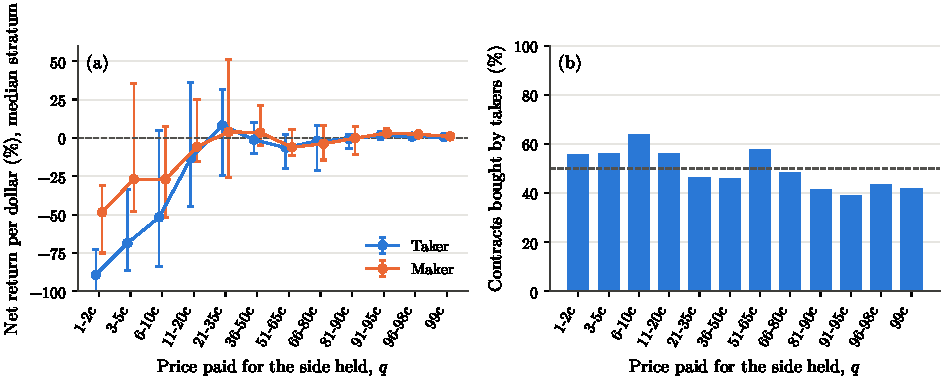
\includegraphics[width=\textwidth]{figures/fig_flow_roles.pdf}
\caption{Takers against makers by the price of the side held. (a) Net return per dollar
(dollar-weighted, after each role's fee) of taker and maker positions: the median across the 18
strata of each stratum's estimate, with bars spanning the interquartile range across strata
(strata with at least five events in the cell). (b) Takers' share of the contracts held at each
price, pooled and design-weighted. Main sample.}\label{fig:flow-roles}
% source: data/research/flb_flow/tables/roles_bucket.csv, roles_bucket_strata.csv
\end{figure}

\begin{table}[htbp]
\centering
\begin{threeparttable}
\caption{Net return per dollar of takers and makers, by group}\label{tab:flow-roles}
\footnotesize
\setlength{\tabcolsep}{4pt}
\begin{tabular}{@{}lrrrrrrr@{}}
\toprule
 & \multicolumn{3}{c}{All positions} & \multicolumn{3}{c}{Longshot positions ($\q\le10\cents$)} & \\
\cmidrule(lr){2-4}\cmidrule(lr){5-7}
Group & Taker & Maker & Difference & Taker & Maker & Taker share & Events \\
\midrule
% source: data/research/flb_flow/tables/roles_overall.csv, roles_diff.csv, roles_side.csv
%BEGIN:roles_group
% source: data/research/flb_flow (generated by flb_flow tex)
Sports & $-2.4$ $(-0.7)$ & $-0.4$ $(-0.1)$ & $-2.0$ $(-0.3)$ & $+52.0$ $(1.0)$ & $+49.9$ $(0.8)$ & $59$ & 1,003 \\
Weather & $-3.0$ $(-2.4)$ & $+1.2$ $(1.3)$ & $-4.2$ $(-1.9)$ & $-15.7$ $(-0.3)$ & $+85.4$ $(0.7)$ & $61$ & 297 \\
Politics & $+1.1$ $(0.6)$ & $-2.1$ $(-1.2)$ & $+3.2$ $(0.9)$ & $-57.2$ $(-3.0)$ & $-37.9$ $(-2.2)$ & $61$ & 258 \\
Entertainment & $+0.3$ $(0.5)$ & $-1.3$ $(-2.3)$ & $+1.6$ $(1.4)$ & $-27.9$ $(-3.1)$ & $-28.4$ $(-2.4)$ & $56$ & 258 \\
Mentions & $-5.1$ $(-2.3)$ & $+1.6$ $(1.7)$ & $-6.8$ $(-2.1)$ & $-62.9$ $(-5.6)$ & $-36.9$ $(-2.2)$ & $76$ & 119 \\
Science \& Tech & $+4.5$ $(5.8)$ & $-7.9$ $(-6.5)$ & $+12.4$ $(6.5)$ & $+92.1$ $(1.5)$ & $-8.2$ $(-0.2)$ & $36$ & 216 \\
\midrule
Non-sports & $-0.9$ $(-1.0)$ & $-0.4$ $(-0.5)$ & $-0.5$ $(-0.3)$ & $-31.0$ $(-1.5)$ & $+11.9$ $(0.3)$ & $60$ & 1,148 \\
All & $-2.4$ $(-0.7)$ & $-0.4$ $(-0.1)$ & $-2.0$ $(-0.3)$ & $+48.9$ $(1.0)$ & $+48.4$ $(0.8)$ & $59$ & 2,151 \\
%END:roles_group
\bottomrule
\end{tabular}
\begin{tablenotes}\footnotesize
\item Main sample, design-weighted. Net return per dollar is dollar-weighted
\eqref{eq:flow-d} after each role's fee, in percent. $t$-statistics clustered by event are in
parentheses. Difference: taker minus maker on the same prints, in percentage points.
Longshot positions are positions in a side bought at $\q\le10\cents$: the taker's side when the
taker bought the longshot, and the maker's side when the taker bought the favourite. Taker share:
the takers' share of longshot contracts held. All pools the groups with design weights and is
dominated by sports.
\end{tablenotes}
\end{threeparttable}
\end{table}

\begin{table}[htbp]
\centering
\begin{threeparttable}
\caption{Longshot positions by stratum: returns, buyers and spreads}\label{tab:flow-strata}
\footnotesize
\setlength{\tabcolsep}{3pt}
\begin{tabular}{@{}lrrrrrrr@{}}
\toprule
 & & \multicolumn{3}{c}{Longshot return (\%/\$)} & \multicolumn{2}{c}{Share at $\q\le10\cents$ (\%)} & Half- \\
\cmidrule(lr){3-5}\cmidrule(lr){6-7}
 & & & & Orders & Orders & Orders & spread \\
Stratum & Events & Takers & Makers & $\le\$100$ & $\le\$10$ & $>\$1$k & (\cents) \\
\midrule
% source: data/research/flb_flow/tables/strata.csv, summary.json (sign_tests)
%BEGIN:strata
% source: data/research/flb_flow (generated by flb_flow tex)
Combat & 59 & $-65$ $(-2.4)$ & $-75$ $(-3.1)$ & $-63$ $(-2.1)$ & $26$ & $0.2$ & $+0.42$ \\
Cricket & 60 & $-57$ $(-1.8)$ & $-36$ $(-0.9)$ & $-59$ $(-2.3)$ & $66$ & $0.8$ & $+0.55$ \\
Esports & 85 & $-86$ $(-8.0)$ & $+37$ $(0.4)$ & $-80$ $(-5.7)$ & $24$ & $0.0$ & $+0.96$ \\
Golf & 30 & $+141$ $(2.1)$ & $+73$ $(1.9)$ & $+218$ $(2.3)$ & $87$ & $36.2$ & $+0.47$ \\
MLB & 87 & $+223$ $(3.9)$ & $+96$ $(1.0)$ & $+191$ $(3.5)$ & $55$ & $2.1$ & $+0.61$ \\
NBA & 49 & $-97$ $(-46.0)$ & $-70$ $(-4.4)$ & $-95$ $(-31.5)$ & $43$ & $0.0$ & $+0.67$ \\
NCAAF & 78 & $-86$ $(-11.6)$ & $-35$ $(-1.1)$ & $-78$ $(-7.0)$ & $38$ & $0.0$ & $+0.29$ \\
NFL & 60 & $-49$ $(-1.5)$ & $+28$ $(0.8)$ & $-63$ $(-3.1)$ & $14$ & $1.0$ & $+0.48$ \\
NHL & 60 & $-84$ $(-8.7)$ & $-59$ $(-1.8)$ & $-80$ $(-6.6)$ & $54$ & $0.0$ & $+0.40$ \\
Other sports & 123 & $-87$ $(-11.4)$ & $-73$ $(-5.7)$ & $-86$ $(-10.3)$ & $77$ & $0.0$ & $+0.34$ \\
Soccer & 113 & $-51$ $(-2.1)$ & $-23$ $(-0.6)$ & $-43$ $(-1.4)$ & $39$ & $0.5$ & $+0.46$ \\
Tennis & 139 & $+55$ $(0.5)$ & $+130$ $(0.7)$ & $+66$ $(0.6)$ & $40$ & $1.5$ & $+0.53$ \\
WNBA & 60 & $-66$ $(-2.8)$ & $-5$ $(-0.2)$ & $-63$ $(-2.5)$ & $31$ & $0.0$ & $-0.11$ \\
\midrule
Entertainment & 258 & $-28$ $(-3.1)$ & $-28$ $(-2.4)$ & $-38$ $(-4.0)$ & $79$ & $0.3$ & $+0.62$ \\
Mentions & 119 & $-63$ $(-5.6)$ & $-37$ $(-2.2)$ & $-69$ $(-6.9)$ & $79$ & $0.2$ & $+0.47$ \\
Politics & 258 & $-57$ $(-3.0)$ & $-38$ $(-2.2)$ & $-39$ $(-1.6)$ & $78$ & $5.0$ & $+0.65$ \\
Science \& Tech & 216 & $+92$ $(1.5)$ & $-8$ $(-0.2)$ & $+72$ $(1.0)$ & $83$ & $3.7$ & $-1.43$ \\
Weather & 297 & $-16$ $(-0.3)$ & $+85$ $(0.7)$ & $-14$ $(-0.3)$ & $70$ & $0.0$ & $+0.71$ \\
\midrule
Sign test, $k/n$ ($p$) & & 14/18 (.015) & 12/18 (.119) & 14/18 (.015) & \multicolumn{2}{c}{18/18 ($<$.001)} & \\
%END:strata
\bottomrule
\end{tabular}
\begin{tablenotes}\footnotesize
\item Main sample, pre-resolution prints. Within a stratum every event has the same design weight, so each row is a
self-weighting random sample. Longshot positions are sides held at $\q\le10\cents$; returns are
dollar-weighted \eqref{eq:flow-d} after each role's fee, with event-clustered $t$-statistics in
parentheses. Shares: the share of taker contracts at $\q\le10\cents$ within taker orders of each size.
Half-spread: the effective half-spread $s$ of taker prints at $\q\le10\cents$ with a tight mid-quote
proxy. Last row: the number $k$ of the $n$ strata with a negative return (for the share columns,
with a larger share in $\le\$10$ orders than in $>\$1$k orders) and the one-sided sign-test
$p$-value.
\end{tablenotes}
\end{threeparttable}
\end{table}

\subsubsection{Trade size: do small takers buy longshots?}\label{sec:res-flow-size}

% source: data/research/flb_flow/tables/size_shares.csv, size_shares_sector.csv, size_side_strata.csv, strata.csv; summary.json (robust, sign_tests)
\paragraph{Small takers buy longshots.} Orders of at most \$10 are 57.8\% of taker orders but
only 5.0\% of taker contracts. Orders above \$1k are 1.1\% of orders and 42.3\% of contracts
(\cref{tab:flow-size}). The share of contracts bought at $\q\le10\cents$ falls steeply with
order size:
\begin{itemize}
  \item 38.9\% in orders of at most \$10;
  \item 17.7\% at \$10--100, 8.5\% at \$100--1k and 1.2\% above \$1k;
  \item the mean price paid rises from 22\cents{} to 59\cents{} across the same size buckets.
\end{itemize}
The gradient is the most robust result of this subsection.
\begin{itemize}
  \item It holds in every one of the 18 strata (sign test $p<0.001$; \cref{tab:flow-strata}).
  \item It holds in both halves of the sample (41\% against 1.1\%, and 37\% against 1.3\%), under
  the strict pre-resolution rule (30\% against 1.5\%) and in the replication sample (62\%
  against 5\%; \cref{tab:flow-robust}).
  \item It is steepest outside sports. In non-sports markets, 74\% of the contracts in orders of
  at most \$10 are longshots, against 2.6\% in orders above \$1k (sports: 36\% against 1.2\%;
  \cref{tab:flow-size-sector}).
\end{itemize}
As a result, orders of at most \$100 place 17.5\% of taker dollars but 59\% of the taker dollars
staked on longshots. Orders above \$1k place 51\% of taker dollars but 8\% of longshot dollars.

\paragraph{Is the loss concentrated in small trades?} In quantity yes, in rate no.
\begin{itemize}
  \item Per dollar, a longshot loses about the same at every size where it can be measured. The
  median-stratum taker return on longshots is $-52\%$ for orders of at most \$10, $-55\%$ at
  \$10--100 and $-52\%$ at \$100--1k (\cref{fig:flow-size}). The full price profile is similar
  for each size bucket (\cref{fig:flow-size-buckets}).
  \item Longshot orders above \$1k are too rare to estimate: only one stratum has five or more
  events with such orders.
  \item Small-order (at most \$100) longshot positions lose in 14 of 18 strata ($p=0.015$).
  \item Favourites earn close to zero at every size.
\end{itemize}
The longshot loss is concentrated in small trades because small trades hold most of the
longshots, not because small traders get worse prices for them. A small order pays the same
half-spread per contract as a large one (\cref{tab:flow-markouts}).

\begin{table}[htbp]
\centering
\begin{threeparttable}
\caption{Taker flow and returns by order size}\label{tab:flow-size}
\footnotesize
\setlength{\tabcolsep}{3.5pt}
\begin{tabular}{@{}lrrrrrrrr@{}}
\toprule
 & \multicolumn{2}{c}{Share of taker} & \multicolumn{2}{c}{Share at $\q\le10\cents$} & & \multicolumn{3}{c}{Taker net return per dollar} \\
\cmidrule(lr){2-3}\cmidrule(lr){4-5}\cmidrule(lr){7-9}
Order size & orders & contracts & contracts & orders & Mean $\q$ (\cents) & Longshots & Favourites & Longshots, per print \\
\midrule
% source: data/research/flb_flow/tables/size_shares.csv, size_side.csv
%BEGIN:size
% source: data/research/flb_flow (generated by flb_flow tex)
$\le$\$10 & $57.8$ & $5.0$ & $38.9$ & $10.5$ & $22$ & $+30.6$ $(0.8)$ & $-2.6$ $(-1.4)$ & $+11.1$ $(0.4)$ \\
\$10--100 & $32.6$ & $21.1$ & $17.7$ & $3.1$ & $35$ & $+52.3$ $(1.1)$ & $-1.3$ $(-0.6)$ & $+44.1$ $(1.2)$ \\
\$100--1k & $8.5$ & $31.7$ & $8.5$ & $1.2$ & $47$ & $+26.1$ $(0.6)$ & $-1.4$ $(-0.6)$ & $+39.0$ $(0.8)$ \\
$>$\$1k & $1.1$ & $42.3$ & $1.2$ & $0.4$ & $59$ & $+164.3$ $(1.2)$ & $-3.6$ $(-0.9)$ & $+67.4$ $(0.7)$ \\
%END:size
\bottomrule
\end{tabular}
\begin{tablenotes}\footnotesize
\item Main sample, all groups, taker positions, design-weighted. Order size is the taker
order's dollar notional (prints with the same market, timestamp and taker side). Shares in
percent. Returns are dollar-weighted \eqref{eq:flow-d} after the taker fee, in percent, with
event-clustered $t$-statistics in parentheses. Per print: each fill weighted equally. Longshots
$\q\le10\cents$; favourites $\q\ge90\cents$.
\end{tablenotes}
\end{threeparttable}
\end{table}

\begin{figure}[htbp]
\centering
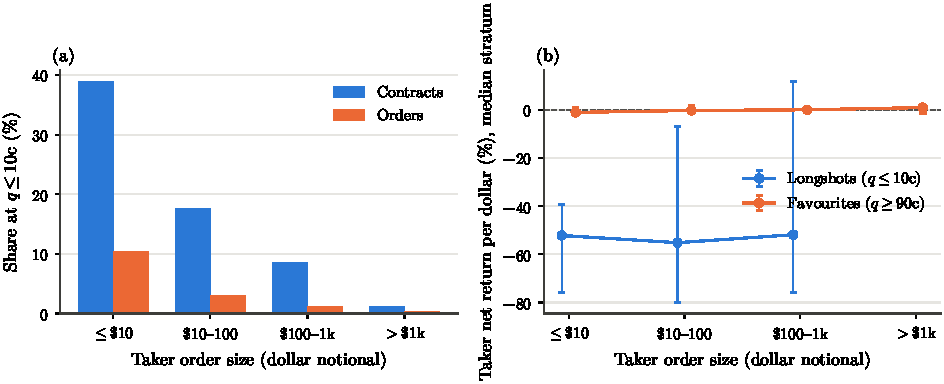
\includegraphics[width=\textwidth]{figures/fig_flow_size.pdf}
\caption{Order size and the longshot. (a) Share of taker contracts and taker orders at
$\q\le10\cents$, by order size, pooled and design-weighted. (b) Taker net return per dollar on
longshots ($\q\le10\cents$) and favourites ($\q\ge90\cents$) by order size: median across strata
with interquartile range, shown where at least six strata have five or more events in the cell
(longshot orders above \$1k qualify in only one stratum). Main sample.}\label{fig:flow-size}
% source: data/research/flb_flow/tables/size_shares.csv, size_side_strata.csv
\end{figure}

\begin{figure}[htbp]
\centering
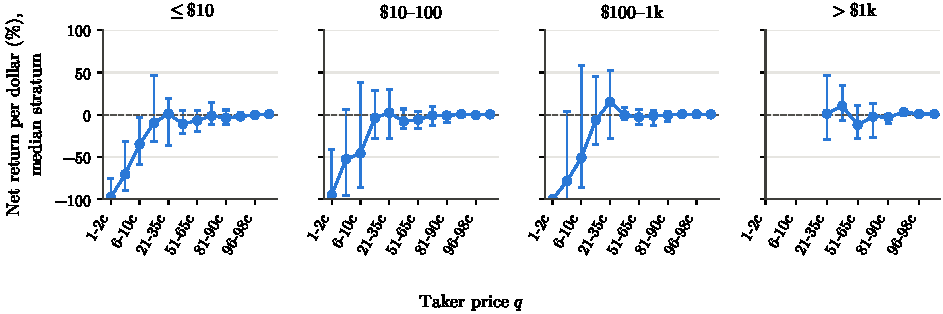
\includegraphics[width=\textwidth]{figures/fig_flow_size_buckets.pdf}
\caption{Taker net return per dollar by price bucket, one panel per order size: median across
strata with interquartile range (cells with at least six qualifying strata). Main sample.}\label{fig:flow-size-buckets}
% source: data/research/flb_flow/tables/size_returns_strata.csv
\end{figure}

\subsubsection{YES and NO takers}\label{sec:res-flow-yesno}

% source: data/research/flb_flow/tables/yesno_share.csv, yesno_strata.csv, yesno_diff.csv; summary.json (yesno_diff_side)
\paragraph{Longshot takers buy YES.} YES accounts for 79--85\% of the taker contracts bought at
$\q\le20\cents$, against 45--53\% at $\q\ge91\cents$ (\cref{tab:flow-yesno}). At equal side
price, YES-takers do worse than NO-takers in 10 of the 12 buckets of the median stratum
(\cref{fig:flow-yesno}). Examples:
\begin{itemize}
  \item at 6--10\cents{}, $-59\%$ against $-14\%$;
  \item at 11--20\cents{}, $-20\%$ against $+27\%$;
  \item at 81--90\cents{}, $-3\%$ against $+5\%$.
\end{itemize}
The pooled differences are significant at 66--80\cents{} ($-20.1$ percentage points, $t=-2.3$)
and 81--90\cents{} ($-25.8$, $t=-3.2$). For favourites as a whole the pooled difference is $-6.2$
points ($t=-1.8$). For longshots it cannot be distinguished from zero ($t=0.1$). There is a YES,
or action, bias, but it is not concentrated in the longshot buckets. The link between the two
biases is compositional: those who buy longshots overwhelmingly buy them as YES.

\begin{figure}[htbp]
\centering
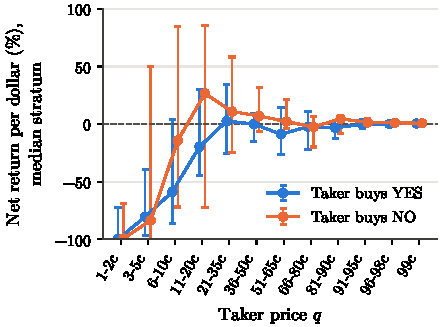
\includegraphics[width=0.55\textwidth]{figures/fig_flow_yesno.pdf}
\caption{Net return per dollar of takers who bought YES and takers who bought NO, at the same
side price: median across strata with interquartile range. Main sample.}\label{fig:flow-yesno}
% source: data/research/flb_flow/tables/yesno_strata.csv
\end{figure}

\subsubsection{Timing and attention}\label{sec:res-flow-timing}

% source: data/research/flb_flow/tables/timing.csv, timing_contrasts.csv
\paragraph{Attention does not bring in more small or longshot flow.} Small orders dominate taker
flow at every hour: about 89\% of taker orders are of at most \$100 throughout the day
(\cref{fig:flow-timing}a; every cell is listed in \cref{tab:flow-timing-cells}). In the classic attention cells (evenings, weekends, primetime games
and marquee events) neither the small-order share nor the longshot share moves significantly
(\cref{fig:flow-timing}b). The busiest cells point the other way.
\begin{itemize}
  \item In volume surges, in play, in a market's first 24 hours and in the last hour before
  expiry, the small-order share \emph{falls}, by 2--4 percentage points ($t$ between $-2.9$ and
  $-5.8$).
  \item During volume surges the longshot share of taker contracts falls by 13 points
  ($t=-2.6$).
\end{itemize}
Surges bring in relatively more large orders and fewer longshot purchases, not a retail rush
into longshots.

\paragraph{Taker returns barely move with attention.} \Cref{tab:flow-timing} compares taker
returns in each attention cell with the rest. Two contrasts are significant.
\begin{itemize}
  \item \emph{Weekends.} Taker returns are $-11.0$ points lower over all positions ($t=-2.3$) and
  $-156$ points lower on longshots ($t=-2.5$).
  \item \emph{The last hour before scheduled expiry.} The bias steepens: longshots do 172 points
  worse ($t=-3.1$) and favourites 9.0 points better ($t=2.2$).
\end{itemize}
Evening, primetime, marquee, in-play, new-listing and surge contrasts are all insignificant, with
wide intervals. Of the 24 return contrasts in \cref{tab:flow-timing}, four have $|t|>2$, and
they fall in only two cells. We therefore do not find that the bias in taker returns widens
systematically when retail attention is high, in the sense of \citet{barberodean2008} and
\citet{barber2022}. The last-hour steepening is the exception: it moves both ends of the bias in
the direction the bias predicts.

\begin{table}[htbp]
\centering
\begin{threeparttable}
\caption{Taker returns in high-attention trading}\label{tab:flow-timing}
\footnotesize
\setlength{\tabcolsep}{4pt}
\begin{tabular}{@{}lrrrrrr@{}}
\toprule
 & \multicolumn{2}{c}{All positions} & \multicolumn{3}{c}{Difference, cell minus rest (pp)} & \\
\cmidrule(lr){2-3}\cmidrule(lr){4-6}
Attention cell & In cell & Rest & All & Longshots & Favourites & Events \\
\midrule
% source: data/research/flb_flow/tables/timing_contrasts.csv
%BEGIN:timing
% source: data/research/flb_flow (generated by flb_flow tex)
Evening, 18--24 ET & $+0.9$ & $-4.4$ & $+5.3$ $(0.9)$ & $-22.3$ $(-0.4)$ & $+2.9$ $(0.6)$ & 2151 \\
Weekend (ET) & $-10.2$ & $+0.7$ & $-11.0$ $(-2.3)$ & $-156.3$ $(-2.5)$ & $+7.5$ $(1.4)$ & 2151 \\
In play (sports) & $-2.6$ & $-3.4$ & $+0.8$ $(0.1)$ & $-57.1$ $(-0.5)$ & $+2.6$ $(0.4)$ & 777 \\
Primetime game (sports) & $-3.1$ & $-2.7$ & $-0.4$ $(-0.1)$ & $-115.2$ $(-1.2)$ & $+6.2$ $(0.9)$ & 777 \\
Marquee event (top decile) & $-2.3$ & $-3.3$ & $+1.0$ $(0.2)$ & $+73.1$ $(1.1)$ & $-4.0$ $(-0.9)$ & 2151 \\
First 24 h after listing & $-5.8$ & $-1.4$ & $-4.5$ $(-0.8)$ & $+64.4$ $(0.6)$ & $-10.4$ $(-1.1)$ & 2151 \\
Volume surge ($\ge 3\times$) & $-1.5$ & $-12.9$ & $+11.3$ $(1.3)$ & $-43.5$ $(-0.5)$ & $+0.1$ $(0.0)$ & 1515 \\
Last hour before expiry & $-5.2$ & $-2.0$ & $-3.3$ $(-0.7)$ & $-172.4$ $(-3.1)$ & $+9.0$ $(2.2)$ & 2151 \\
%END:timing
\bottomrule
\end{tabular}
\begin{tablenotes}\footnotesize
\item Main sample, all groups, taker positions, design-weighted. Net return per dollar is
dollar-weighted \eqref{eq:flow-d} after the taker fee, in percent. Differences are in
percentage points, with event-clustered $t$-statistics in parentheses. In-play and primetime
contrasts are within sports games with a known scheduled start. A volume surge means the
market's volume in the preceding hour is at least three times its own past hourly average.
Marquee: the event's total volume is in the top decile of its stratum (ex post).
\end{tablenotes}
\end{threeparttable}
\end{table}

\begin{figure}[htbp]
\centering
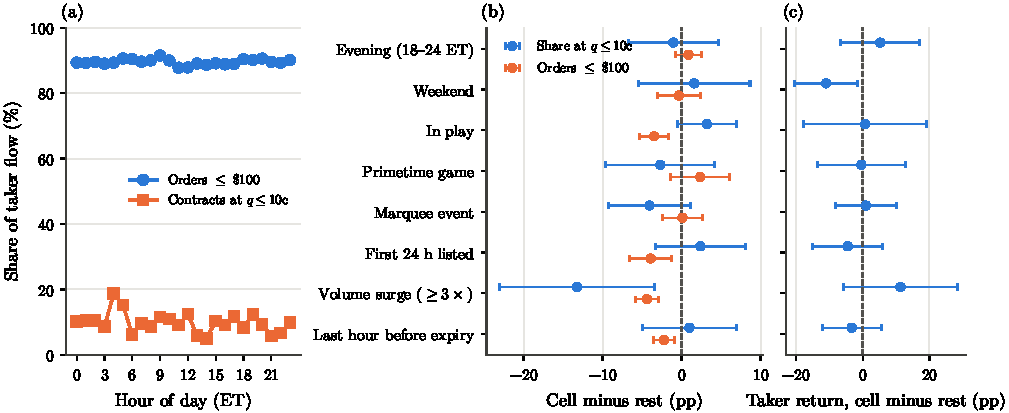
\includegraphics[width=\textwidth]{figures/fig_flow_timing.pdf}
\caption{Timing and attention. (a) Share of taker orders of at most \$100 and share of taker
contracts at $\q\le10\cents$, by hour of day (ET). (b) Each attention cell minus the rest: the
share of taker contracts at $\q\le10\cents$ and the share of taker orders of at most \$100, in
percentage points. (c) Each attention cell minus the rest: taker net return per dollar over all
positions. 95\% confidence intervals clustered by event. Main sample, design-weighted.}\label{fig:flow-timing}
% source: data/research/flb_flow/tables/timing.csv, timing_contrasts.csv
\end{figure}

\subsubsection{Order flow, price impact and information}\label{sec:res-flow-impact}

% source: data/research/flb_flow/tables/markouts.csv, markouts_strata.csv, decomp_side.csv; summary.json (hourly, markouts_coverage)
\paragraph{Price impact rises with size.} These results use the prints with a tight mid-quote
proxy before and after the order: 36\% of contracts, concentrated in the more liquid markets.
\begin{itemize}
  \item Every size bucket pays a similar effective half-spread, 0.56--0.68\cents{} per contract
  ($t>16$; \cref{tab:flow-markouts}).
  \item One minute after the order, the mid has moved in the taker's direction by 0.04\cents{}
  for orders of at most \$10 and by 0.41\cents{} for orders above \$1k ($t$ from 2.5 to 4.9).
  \item One hour later, the median-stratum impact is 0.20, 0.66, 1.78 and 0.39\cents{} across
  the four size buckets.
\end{itemize}

\paragraph{Market-hour order flow.} Regression~\eqref{eq:flow-reg} uses the 15,740
market-hours, in 651 events, with a tight proxy at both ends of the hour (\cref{tab:flow-oib},
\cref{fig:flow-impact}).
\begin{itemize}
  \item \emph{Same hour.} An hour of entirely one-sided taker flow moves the mid by 0.28\cents{}
  if it is small ($t=2.6$), 2.74\cents{} if medium ($t=7.4$) and 3.26\cents{} if large
  ($t=5.3$).
  \item \emph{Next hour.} Small and medium flow keep moving the price in the same direction
  (0.35\cents, $t=2.8$; 0.58\cents, $t=2.6$). The impact of large flow neither continues nor
  reverts ($-0.08$\cents, $t=-0.2$), while the mid itself partly reverses (coefficient on the
  same-hour change $-0.12$, $t=-2.2$).
  \item \emph{To settlement.} No size class predicts the outcome. The estimates are 3.3\cents{}
  for small flow ($t=1.3$), $-0.4\cents$ for medium ($t=-0.3$) and $-11.3\cents$ for large
  ($t=-1.6$).
\end{itemize}

\paragraph{Small flow is neither informed nor noise that reverts.} Small taker flow moves prices
little and does not predict outcomes, but its impact does not reverse within the hour either.
This differs from equity markets, where the net buying of individual investors predicts
returns over the following weeks \citep{kanielsaartitman2008,boehmer2021}.
Large flow moves prices most, as the depth of a \citet{kyle1985} market implies, but the
outcome does not confirm its direction. If anything, the point estimate goes against it, in
sports and non-sports alike. The per-order markouts to settlement are noisy and centred near
zero (median stratum between $-0.7$ and $+2.7\cents$). Combined with the immediacy cost above,
this explains the taker's loss on longshots as a liquidity cost, not as adverse selection
against informed makers. Takers lose because they pay the spread and the fee on cheap
contracts. They do not lose because the side they buy predictably moves against them.

\begin{table}[htbp]
\centering
\begin{threeparttable}
\caption{Price impact and markouts of taker orders by size (cents per contract)}\label{tab:flow-markouts}
\footnotesize
\begin{tabular}{@{}lrrrrr@{}}
\toprule
Order size & Half-spread $s$ & Impact $I_{1m}$ & Impact $I_{1h}$ & Markout $M_{1h}$ & Markout $M_\infty$ \\
\midrule
% source: data/research/flb_flow/tables/markouts.csv
%BEGIN:markouts
% source: data/research/flb_flow (generated by flb_flow tex)
$\le$\$10 & $+0.56$ $(21.2)$ & $+0.04$ $(2.5)$ & $+3.43$ $(2.6)$ & $+2.87$ $(2.1)$ & $+21.69$ $(1.7)$ \\
\$10--100 & $+0.58$ $(19.6)$ & $+0.10$ $(3.5)$ & $+2.91$ $(2.3)$ & $+2.33$ $(1.8)$ & $+13.28$ $(1.3)$ \\
\$100--1k & $+0.68$ $(18.3)$ & $+0.19$ $(4.9)$ & $+1.03$ $(1.6)$ & $+0.35$ $(0.5)$ & $+2.18$ $(0.5)$ \\
$>$\$1k & $+0.68$ $(16.8)$ & $+0.41$ $(4.1)$ & $-1.40$ $(-1.4)$ & $-2.08$ $(-2.1)$ & $-6.86$ $(-0.8)$ \\
%END:markouts
\bottomrule
\end{tabular}
\begin{tablenotes}\footnotesize
\item Main sample, all groups, taker prints with a mid-quote proxy no wider than 5\cents{} just
before the order and a proxy one minute and one hour after it. Contract-weighted and design-weighted, in cents per contract, from
the taker's side \eqref{eq:flow-markout}. $M_\infty$ is the gross profit to settlement. $t$-statistics
clustered by event are in parentheses.
\end{tablenotes}
\end{threeparttable}
\end{table}

\begin{table}[htbp]
\centering
\begin{threeparttable}
\caption{Spread or price? Decomposing the taker's gross loss (cents per contract)}\label{tab:flow-decomp}
\footnotesize
\setlength{\tabcolsep}{4pt}
\begin{tabular}{@{}llrrrrrr@{}}
\toprule
 & & Mean $\q$ & Gross profit & Mid to outcome & Half-spread & Fee & Immediacy \\
Sample & Taker side & (\cents) & $d(Y-p)$ & $d(Y-m_{t^-})$ & $s$ & $\fee^T$ & cost (\%/\$) \\
\midrule
% source: data/research/flb_flow/tables/decomp_side.csv
%BEGIN:decomp
% source: data/research/flb_flow (generated by flb_flow tex)
Sports & Longshots ($\q\le10\cents$) & $5.5$ & $+2.00$ $(0.6)$ & $+2.51$ $(0.8)$ & $+0.50$ $(14.0)$ & $0.33$ & $14.2$ \\
 & Middle & $49.4$ & $-0.15$ $(-0.1)$ & $+0.64$ $(0.3)$ & $+0.78$ $(13.0)$ & $1.34$ & $4.2$ \\
 & Favourites ($\q\ge90\cents$) & $94.9$ & $-2.52$ $(-0.6)$ & $-1.51$ $(-0.4)$ & $+1.02$ $(11.0)$ & $0.32$ & $1.4$ \\
Non-sports & Longshots ($\q\le10\cents$) & $3.8$ & $-0.17$ $(-0.1)$ & $+0.45$ $(0.3)$ & $+0.62$ $(11.7)$ & $0.25$ & $21.2$ \\
 & Middle & $47.8$ & $+1.61$ $(0.9)$ & $+3.94$ $(2.8)$ & $+2.34$ $(6.0)$ & $1.31$ & $7.4$ \\
 & Favourites ($\q\ge90\cents$) & $96.9$ & $-2.05$ $(-0.6)$ & $+0.56$ $(0.2)$ & $+2.61$ $(5.3)$ & $0.21$ & $2.9$ \\
All & Longshots ($\q\le10\cents$) & $5.5$ & $+1.94$ $(0.6)$ & $+2.44$ $(0.8)$ & $+0.51$ $(14.4)$ & $0.33$ & $14.4$ \\
 & Middle & $49.4$ & $-0.14$ $(-0.1)$ & $+0.65$ $(0.3)$ & $+0.79$ $(12.8)$ & $1.34$ & $4.2$ \\
 & Favourites ($\q\ge90\cents$) & $95.0$ & $-2.51$ $(-0.6)$ & $-1.44$ $(-0.4)$ & $+1.07$ $(10.8)$ & $0.32$ & $1.5$ \\
%END:decomp
\bottomrule
\end{tabular}
\begin{tablenotes}\footnotesize
\item Main sample, taker prints with a mid-quote proxy no wider than 5\cents{} just before the
order. Contract-weighted and design-weighted, in cents per contract, with event-clustered
$t$-statistics in parentheses. By construction the gross profit equals the mid-to-outcome term
minus the half-spread. The first term is the bias in the quoted price that any buyer of the
side faces, and the second is the cost of immediacy. Fee: the exact taker fee per contract.
Immediacy cost: $(s+\fee^T)/(\q+\fee^T)$, dollar-weighted, in percent of the stake.
\end{tablenotes}
\end{threeparttable}
\end{table}

\begin{table}[htbp]
\centering
\begin{threeparttable}
\caption{Signed taker imbalance by size class and subsequent mid-quote changes}\label{tab:flow-oib}
\footnotesize
\setlength{\tabcolsep}{4pt}
\begin{tabular}{@{}llrrrrrr@{}}
\toprule
 & & \multicolumn{3}{c}{Imbalance $\mathrm{OIB}_c$} & Same-hour & Market- & \\
\cmidrule(lr){3-5}
Sample & Change & Small & Medium & Large & change & hours & Events \\
\midrule
% source: data/research/flb_flow/summary.json (hourly)
%BEGIN:oib
% source: data/research/flb_flow (generated by flb_flow tex)
All & Same hour & $+0.28$ $(2.6)$ & $+2.74$ $(7.4)$ & $+3.26$ $(5.3)$ & -- & 15,740 & 651 \\
 & Next hour & $+0.35$ $(2.8)$ & $+0.58$ $(2.6)$ & $-0.08$ $(-0.2)$ & $-0.12$ $(-2.2)$ & 9,611 & 381 \\
 & To settlement & $+3.28$ $(1.3)$ & $-0.45$ $(-0.3)$ & $-11.26$ $(-1.6)$ & $+0.01$ $(0.2)$ & 15,740 & 651 \\
Sports & Same hour & $-0.63$ $(-1.3)$ & $+1.84$ $(3.6)$ & $+2.87$ $(3.6)$ & -- & 3,281 & 308 \\
 & Next hour & $+0.66$ $(1.1)$ & $+0.33$ $(0.7)$ & $-0.06$ $(-0.1)$ & $-0.43$ $(-2.6)$ & 2,084 & 173 \\
 & To settlement & $+8.24$ $(1.2)$ & $+1.20$ $(0.2)$ & $-6.50$ $(-0.8)$ & $+0.02$ $(0.3)$ & 3,281 & 308 \\
Non-sports & Same hour & $+0.45$ $(4.0)$ & $+3.11$ $(5.9)$ & $+3.64$ $(3.8)$ & -- & 12,459 & 343 \\
 & Next hour & $+0.25$ $(2.1)$ & $+0.44$ $(1.8)$ & $+0.05$ $(0.2)$ & $-0.02$ $(-0.4)$ & 7,527 & 208 \\
 & To settlement & $+2.61$ $(1.0)$ & $-0.76$ $(-0.5)$ & $-13.50$ $(-1.4)$ & $+0.00$ $(0.1)$ & 12,459 & 343 \\
%END:oib
\bottomrule
\end{tabular}
\begin{tablenotes}\footnotesize
\item OLS of regression~\eqref{eq:flow-reg} on market-hours with taker volume and a tight
($\le5\cents$) mid-quote proxy at both ends of the hour (and of the next hour, for the next-hour
change). The dependent
variable is in cents. The imbalances~\eqref{eq:flow-oib} are signed contracts of each size
class (small $\le\$100$, medium $\$100$--$1$k, large $>\$1$k) over the hour's volume. Same-hour
change: the control $m^{\mathrm{end}}_h-m^{\mathrm{start}}_h$. $t$-statistics (CR1, clustered
by event) are in parentheses. Market-hours are unweighted.
\end{tablenotes}
\end{threeparttable}
\end{table}

\begin{figure}[htbp]
\centering
\begin{subfigure}[t]{0.58\textwidth}
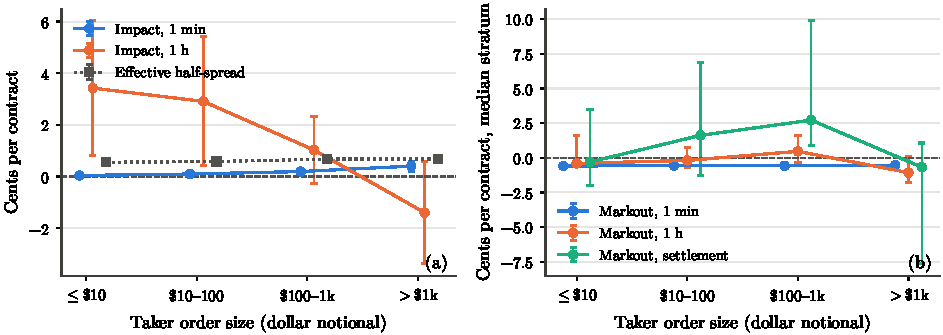
\includegraphics[width=\textwidth]{figures/fig_flow_markouts.pdf}
\end{subfigure}
\hfill
\begin{subfigure}[t]{0.40\textwidth}
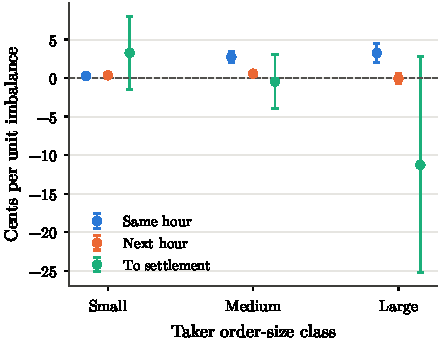
\includegraphics[width=\textwidth]{figures/fig_flow_oib.pdf}
\end{subfigure}
\caption{Price impact and information. Left: (a) effective half-spread and price impact at
one minute and one hour (pooled, design-weighted, 95\% intervals clustered by event), and (b)
taker markouts at one minute, one hour and settlement (median across strata with interquartile
range), by taker order size, in cents per contract. Right: coefficients of
regression~\eqref{eq:flow-reg} on the signed imbalance of each size class, for the same-hour
change, the next-hour change and the drift to settlement, with 95\% intervals clustered by
event.}\label{fig:flow-impact}
% source: data/research/flb_flow/tables/markouts.csv, markouts_strata.csv, summary.json (hourly)
\end{figure}

\subsubsection{Robustness}\label{sec:res-flow-robust}

% source: data/research/flb_flow/summary.json (robust, sign_tests)
\Cref{tab:flow-robust} repeats the headline numbers in subsamples. The results that hold
everywhere are the size gradient in longshot buying and the absence of a taker--maker gap
averaged over all prices.
\begin{itemize}
  \item \emph{Size gradient.} The longshot share of orders of at most \$10 exceeds that of
  orders above \$1k by 28 to 57 points in both halves, under the strict rule and in the
  replication sample.
  \item \emph{No overall taker--maker gap.} Pooled taker returns lie between $-0.9$ and
  $-3.5\%$ and maker returns between $-1.4$ and $+0.5\%$. Neither is significant in any
  variant. Clustering by market instead of event leaves the difference insignificant
  ($t=-0.1$).
  \item \emph{Pooled longshot returns are unstable.} The pooled taker return on longshots is
  $-35\%$ in the first half and $+125\%$ in the second. The second half contains the MLB
  home-run prop that dominates the pooled sports estimate.
  \item \emph{Small-order longshots.} Without design weights, longshot positions in orders of at
  most \$10 lose 28\% ($t=-2.2$). In the replication sample, which is a much larger set of
  prints, they lose 37\% ($t=-1.9$).
  \item \emph{Excluded prices.} Dropping 1--2\cents{} and 99\cents{} prints changes nothing
  material.
\end{itemize}

\begin{table}[htbp]
\centering
\begin{threeparttable}
\caption{Headline results across subsamples and weights}\label{tab:flow-robust}
\footnotesize
\setlength{\tabcolsep}{3.5pt}
\begin{tabular}{@{}lrrrrrr@{}}
\toprule
 & \multicolumn{2}{c}{All positions} & \multicolumn{3}{c}{Taker longshots ($\q\le10\cents$)} & \LS{} share (\%) \\
\cmidrule(lr){2-3}\cmidrule(lr){4-6}
Sample & Taker & Maker & All orders & $\le\$10$ orders & $>\$1$k orders & $\le\$10$ / $>\$1$k \\
\midrule
% source: data/research/flb_flow/summary.json (headline, robust)
%BEGIN:robust
% source: data/research/flb_flow (generated by flb_flow tex)
Main sample & $-2.4$ $(-0.7)$ & $-0.4$ $(-0.1)$ & $+48.9$ $(1.0)$ & $+30.6$ $(0.8)$ & $+164.3$ $(1.2)$ & $39$ / $1$ \\
First half (by close) & $-1.2$ $(-0.2)$ & $-1.4$ $(-0.2)$ & $-34.9$ $(-1.1)$ & $-30.2$ $(-1.0)$ & $-99.9$ $(-1853.9)$ & $41$ / $1$ \\
Second half & $-3.5$ $(-1.3)$ & $+0.5$ $(0.2)$ & $+124.8$ $(1.7)$ & $+75.2$ $(1.3)$ & $+323.5$ $(1.6)$ & $37$ / $1$ \\
Strict pre-resolution & $-3.1$ $(-0.3)$ & $+0.1$ $(0.0)$ & $+105.9$ $(1.2)$ & $+109.4$ $(1.3)$ & $+65.3$ $(0.4)$ & $30$ / $2$ \\
Excluding 1--2\cents{} and 99\cents & $-2.5$ $(-0.7)$ & $-0.4$ $(-0.1)$ & $+50.5$ $(1.0)$ & $+39.9$ $(0.8)$ & $+164.4$ $(1.2)$ & $27$ / $1$ \\
No design weights & $-2.1$ $(-1.2)$ & $-0.3$ $(-0.2)$ & $-8.0$ $(-0.4)$ & $-28.4$ $(-2.2)$ & $-1.2$ $(-0.0)$ & $57$ / $2$ \\
Sports & $-2.4$ $(-0.7)$ & $-0.4$ $(-0.1)$ & $+52.0$ $(1.0)$ & $+36.1$ $(0.8)$ & $+169.0$ $(1.2)$ & $36$ / $1$ \\
Non-sports & $-0.9$ $(-1.0)$ & $-0.4$ $(-0.5)$ & $-31.0$ $(-1.5)$ & $-35.2$ $(-1.3)$ & $-85.1$ $(-4.6)$ & $74$ / $3$ \\
Replication sample & $-3.0$ $(-0.7)$ & $+0.2$ $(0.1)$ & $+6.2$ $(0.2)$ & $-36.6$ $(-1.9)$ & $+40.3$ $(0.7)$ & $62$ / $5$ \\
Replication, strict & $-3.2$ $(-0.8)$ & $+0.4$ $(0.1)$ & $+12.5$ $(0.4)$ & $-24.2$ $(-1.0)$ & $-5.5$ $(-0.1)$ & $52$ / $5$ \\
%END:robust
\bottomrule
\end{tabular}
\begin{tablenotes}\footnotesize
\item Net return per dollar, dollar-weighted \eqref{eq:flow-d} after each role's fee, in
percent, with event-clustered $t$-statistics in parentheses. Halves split the main sample's
markets at their median close time. Strict pre-resolution keeps only pre-game sports prints and
other prints more than 24 hours before the close. The replication sample is the separate set
of prints described in \cref{sec:data-flow}, which carries no design weights. \LS{} share: the
share of taker contracts at $\q\le10\cents$ in orders of at most \$10 and of more than \$1k.
\end{tablenotes}
\end{threeparttable}
\end{table}

\paragraph{Summary.} The trade-level evidence partly supports the preference and retail-demand
hypothesis (\cref{hyp:pref}).
\begin{itemize}
  \item Small takers are the longshot buyers. The size gradient holds in every stratum, and
  takers buy most longshots, mainly as YES.
  \item Takers lose more than makers on longshots. They pay a spread and a fee that together
  cost about 14\% of the stake at the average longshot price of 5.5\cents.
  \item But the per-dollar loss on a longshot is about the same for small and larger orders, and
  attention does not systematically widen it.
\end{itemize}
The information hypothesis (\cref{hyp:info}) finds no support at the trade level. Neither small
nor large taker flow predicts outcomes beyond the price. The resting side of a longshot trade
earns the spread; it is not exploiting the taker's ignorance of the outcome. Who pays the bias is
therefore mostly a question of who demands immediacy on cheap contracts, and on Kalshi that is
small takers.
